% ============================================================
%  Section 2: BERT Architecture
% ============================================================

\section{BERT Architecture}
\label{sec:architecture}

\bert{} is built exclusively upon the \emph{encoder} stack of the original
Transformer architecture proposed by Vaswani~et~al.~\cite{vaswani2017attention}.
Unlike the full encoder-decoder Transformer used for sequence-to-sequence tasks,
\bert{} discards the decoder entirely; its objective is to produce rich contextual
representations of input tokens rather than to autoregressively generate output
sequences.

\subsection{Transformer Encoder Stack}
\label{subsec:encoder}

The model consists of $L$ identical encoder layers stacked sequentially.  Each
layer $\ell \in \{1, \ldots, L\}$ transforms its input representation
$\mathbf{H}^{(\ell-1)} \in \R^{n \times d}$ (where $n$ is the sequence length and
$d$ is the hidden dimension) into a refined output $\mathbf{H}^{(\ell)}$ through
two principal sub-layers:

\begin{enumerate}
  \item \textbf{Multi-Head Self-Attention~(MHSA).}  Tokens attend to all other
        tokens in the sequence, producing context-enriched representations.
        (Described in detail in \cref{sec:attention}.)

  \item \textbf{Position-Wise Feed-Forward Network~(FFN).}  A pair of linear
        transformations with a $\gelu$ non-linearity is applied independently to
        each token position.
\end{enumerate}

\noindent Both sub-layers are wrapped with \emph{residual connections} and
\emph{layer normalisation}~\cite{ba2016layer}, following the formulation:
\begin{equation}
  \mathbf{H}^{(\ell)} = \operatorname{LayerNorm}\!\bigl(
    \mathbf{z} + \operatorname{SubLayer}(\mathbf{z})
  \bigr), \quad \mathbf{z} = \mathbf{H}^{(\ell-1)}.
  \label{eq:residual}
\end{equation}
Residual connections mitigate the vanishing-gradient problem and stabilise training
in deep networks, while layer normalisation normalises activations across the hidden
dimension for each token independently.

\begin{table}[H]
  \centering
  \caption{Computation flow within a single Transformer encoder layer.  MHSA denotes
           Multi-Head Self-Attention; FFN denotes Position-Wise Feed-Forward Network.}
  \label{tab:layer_composition}
  \renewcommand{\arraystretch}{1.4}
  \begin{tabular}{lcc}
    \toprule
    \textbf{Sub-layer} & \textbf{Input} & \textbf{Output Dimension} \\
    \midrule
    MHSA  & $\mathbf{H}^{(\ell-1)} \in \mathbb{R}^{n \times d}$ & $\mathbb{R}^{n \times d}$ \\
    \hspace{0.5cm} + LayerNorm + Residual & & \\
    FFN   & $\mathbf{H}^{(\ell)} \in \mathbb{R}^{n \times d}$ & $\mathbb{R}^{n \times d}$ \\
    \hspace{0.5cm} + LayerNorm + Residual & & \\
    \bottomrule
  \end{tabular}
\end{table}

\begin{figure}[H]
  \centering
  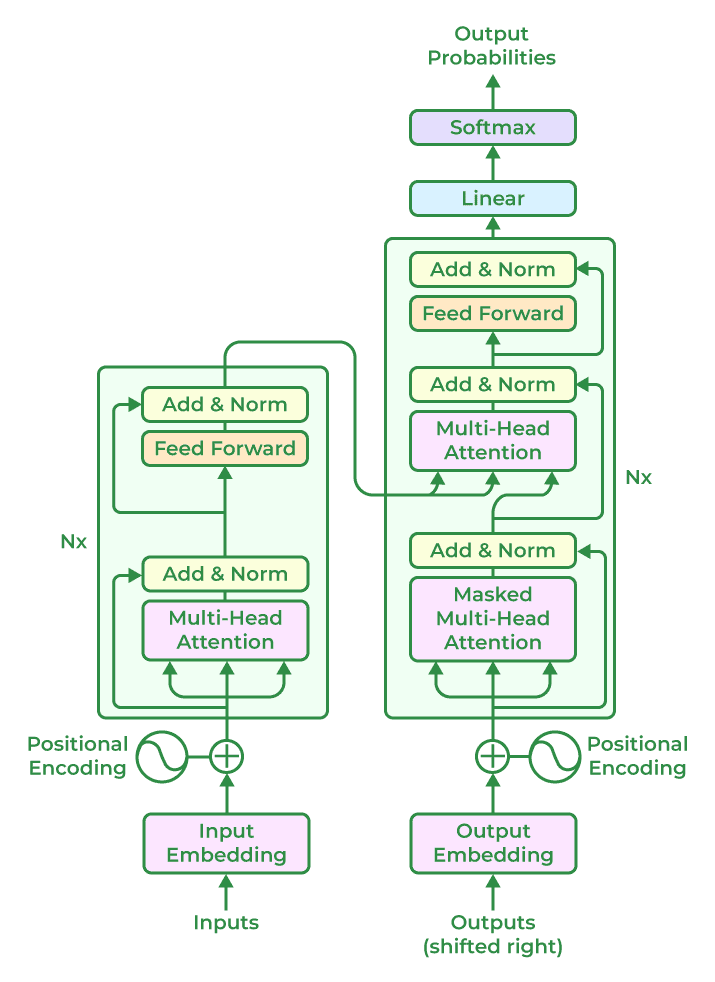
\includegraphics[width=0.72\textwidth]{figures/transformer.png}
  \caption{Stacked Transformer encoder architecture underlying \bert{}.  Each of the
           $L$ encoder layers applies Multi-Head Attention followed by a Feed-Forward
           Network, with residual connections and layer normalisation at each
           sub-layer.}
  \label{fig:transformer}
\end{figure}

\subsection{Hierarchical Representation Learning}
\label{subsec:hierarchical}

A salient property of deep Transformer encoders is their ability to construct
\emph{hierarchical} representations across layers.

\begin{itemize}
  \item \textbf{Lower layers} ($\ell \approx 1$--$4$) tend to encode surface-level
        and syntactic information such as part-of-speech tags, morphology, and
        local phrase structure~\cite{tenney2019bert}.

  \item \textbf{Middle layers} ($\ell \approx 5$--$8$) capture syntactic
        dependencies including subject-verb agreement and coreference.

  \item \textbf{Upper layers} ($\ell \approx 9$--$12$ for \bert{}-Base) encode
        high-level semantic information and task-relevant abstractions, making them
        particularly well-suited as features for downstream tasks.
\end{itemize}

This layered abstraction mirrors the hierarchical feature extraction observed in
convolutional neural networks applied to vision tasks, and it affords \bert{} the
ability to generalise across a broad range of linguistic phenomena.

\subsection{Model Configurations}
\label{subsec:configs}

Two standard configurations of \bert{} were released, differing in depth and width:

\begin{table}[H]
  \centering
  \caption{Standard \bert{} model configurations.  $L$: number of encoder layers;
           $H$: hidden dimension; $A$: number of attention heads;
           $P$: total parameter count.}
  \label{tab:configs}
  \renewcommand{\arraystretch}{1.25}
  \begin{tabular}{lcccc}
    \toprule
    \textbf{Variant} & $L$ & $H$ & $A$ & $P$ \\
    \midrule
    \bert{}-Base  & 12 & 768  & 12 & $\approx$110M \\
    \bert{}-Large & 24 & 1024 & 16 & $\approx$340M \\
    \bottomrule
  \end{tabular}
\end{table}

\bert{}-Large achieves higher performance on most benchmarks but demands
substantially greater computational resources for both pre-training and fine-tuning.
\bert{}-Base remains the standard choice for resource-constrained settings.
